\section{Méthode des puissances}
	
	\subsection{Algorithme}
	
		\begin{adjustwidth}{1.5cm}{1.5cm} 
		\begin{algorithm}[H]
			\caption{Méthode des puissances}
			\Donnees{Vecteur $\Pi$ de pertinence de taille $n$, Matrice du web $M$, $e$ vecteur de $1$ de taille $n$}
			$k \gets 0$ \text{ et }
			$\Pi^{(k)} \gets \frac{1}{n} \cdot e$\; 
			\Repeter{ $\| \Pi^{(k + 1)} - \Pi^{(k)} \|_{1} > \epsilon$ }{
				$k \gets k + 1$\;
				\Pour{$i \gets 1$ allant à $n$}{
					$\Pi^{(k)}[i] \gets \alpha \cdot (\sum_{j = 1}^{n} \Pi^{(k - 1)}[j] \cdot M[j,i]) + \frac{1 - \alpha}{n} + \frac{\sigma \cdot \alpha}{n}$\;
				}
			}
		\end{algorithm}
		\end{adjustwidth}
		
		\paragraph{}$\alpha = 0.85$, $\epsilon = 10^{-6}$,  $\sigma = \frac{f^{T} \cdot e}{n}$ et $f$ le vecteur ligne tel que $f[i]$ vaut $1$ si le degré sortant du noeur $i$ de $M$ est nul et $0$ sinon.
		\paragraph{}Les distributions obtenues avec notre algorithme ont pu être vérifiées sur de petits graphes à l'aide du logiciel Scilab :\\
		\begin{center}
			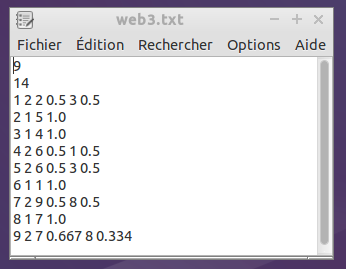
\includegraphics[scale=0.5]{matrice.png}
			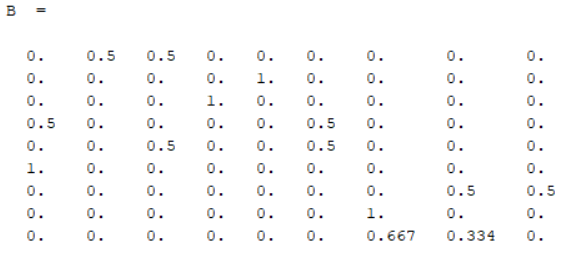
\includegraphics[scale=0.5]{matriceScilab.png}
			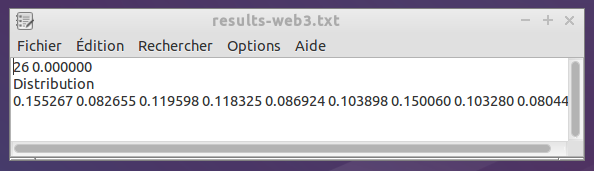
\includegraphics[scale=0.7]{distrib.png}
			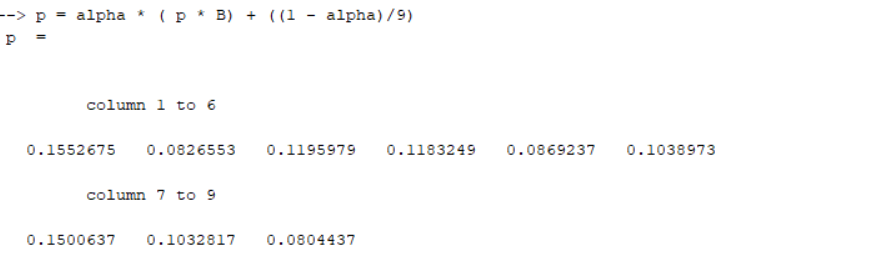
\includegraphics[scale=0.5]{distribScilab.png}
		\end{center}
		
	\subsection{Principe}
	
		\paragraph{}L'algorithme effectue des multiplications vecteur-matrice à répétitions, cela dit, nous n'utilisons pas directement la matrice du web, mais on effectue deux transformations.
		\paragraph{}La première transformation, $M^{'} \gets M + \frac{f^{T} \cdot e}{n}$ , vise à rendre la matrice du web stochastique. C'est un élément critique pour justifier la convergence de l'algorithme.
		\paragraph{}La deuxième transformation, $G \gets \alpha \cdot M^{'} + (1 - \alpha) \cdot \frac{e^{T} \cdot e}{n}$ , ajoute un bruit à la matrice pour accélérer la convergence de l'algorithme.

	\subsection{Complexité}
		
		\paragraph{}En ce qui concerne la complexité, nous allons simplement énoncer ici que le nombre d'itérations de la boucle \textit{do-while} de l'algorithme dépend de la convergence de la suite $\Pi^{(k + 1)} = \Pi^{(k)} \cdot M$.
		\paragraph{}Soit $\{\lambda_{1}, \cdots, \lambda_{n} \}$ l'ensemble des valeurs propres de $M$ trié par valeur décroissante. La suite des $(\Pi^{(k)})_{n \in \mathbb{N}}$ se comporte comme une suite géométrique de raison $\lambda_{2}$. Ainsi, après la transformation de $M$ en la matrice $G$, on peut prouver que la convergence est accélérée en $\alpha \cdot \lambda_{2}$.
